\documentclass[a4paper]{article}
\usepackage{tikz}
\usepackage{amssymb}
\usetikzlibrary{mindmap, automata, positioning, arrows}

\begin{document}

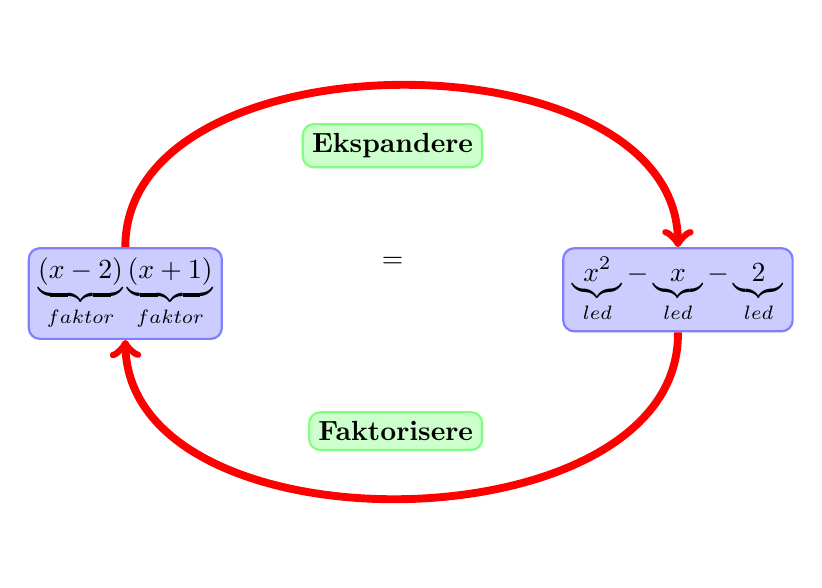
\begin{tikzpicture}
  [eq/.style={rectangle,rounded corners,draw=blue!50,fill=blue!20,thick},
ac/.style={rectangle,rounded corners,draw=green!50,fill=green!20,thick}]

  \node[eq] (leq) 
                             {$\underbrace{(x-2)}_{faktor}\underbrace{(x+1)}_{faktor}$};
  \node[ac] (exp)   [above right=of leq] {\textbf{Ekspandere}};
  \node      (equal) [below =of exp] {$=$};
  \node[eq]  (req)  [below right=of exp] 
                            {$\underbrace{x^2}_{led} -\underbrace{x}_{led} -\underbrace{2}_{led}$};
  \node[ac] (exp) [below left=of req] {\textbf{Faktorisere}};

\path [->,line width=0.1cm,red] (req.south)  edge [bend left=90] (leq.south);
\path [->,line width=0.1cm,red] (leq.north)  edge [bend left=90] (req.north);

\end{tikzpicture}


\end{document}